\documentclass{article}
\usepackage{graphicx}
\usepackage{amsmath,amssymb,amsthm}
\usepackage{parskip}
\usepackage{float}
\usepackage[margin=0.5in]{geometry}

% Theorem definitions
\newtheorem{theorem}{Theorem}[section]
\newtheorem{corollary}{Corollary}[theorem]
\newtheorem{lemma}[theorem]{Lemma}
\newtheorem{remark}{Remark}
\newtheorem{note}{Note}
\renewcommand{\qedsymbol}{$\blacksquare$}

% Fix theorem spacing
\makeatletter
\def\thm@space@setup{%
  \thm@preskip=\parskip \thm@postskip=0pt
}
\makeatother

% Equation numbering
\newcommand\numberthis{\addtocounter{equation}{1}\tag{\theequation}}

% Vector utils
\renewcommand{\vec}[1]{\boldsymbol{#1}}
\newcommand{\rvec}[1]{\begin{bmatrix} #1 \end{bmatrix}}
\newcommand{\norm}[1]{\left\lVert#1\right\rVert}

\begin{document}

\title{LCP Notes}
\author{Samuel Pfrommer}

\maketitle

\section{Falling block}
Consider a block of unit mass falling from an arbitrary height onto a static surface under the influence of a gravitational force with constant $-g$. We then have the following equations of motion:
\begin{align*}
    x_{k+1} &= x_k + \dot x_{k+1} \Delta t \\
    \dot x_{k+1} &= \dot x_k + (-g + \lambda _{k+1}) \Delta t
\end{align*}

Where $x_n$ represents the separation of the block from the surface at time step $n$, $\lambda_n$ is the nonpenetration contact force, and $\Delta t$ is our discrete time step. Note we are using implicit euler to prevent penetration of the block with the surface. Substituting the second equation into the first we have:
\begin{align*}
    x_{k+1} &= x_k + (\dot x_k + (-g + \lambda _{k+1}) \Delta t) \Delta t \\
    x_{k+1} &= x_k + \dot x_k \Delta t + -g \Delta t ^2 + \lambda _{k+1} \Delta t ^2 \\
    \lambda_{k+1} &= \frac{1}{\Delta t^2} x_{k+1} - \frac{1}{\Delta t^2} x_k - \frac{1}{\Delta t} \dot x_k + g \\
    \lambda_{k+1} &= \frac{1}{\Delta t^2} x_{k+1} - \frac{1}{\Delta t^2} (x_k + \Delta t \dot x_k - g \Delta t^2)
\end{align*}

Observe that we solve an LCP for each time step, and as such $x_k$ and $\dot x_k$ are given to us from the previous time step. The problem therefore consists of solving for $x_{k+1}$, $\dot x_{k+1}$, and $\lambda_{k+1}$. Since $\lambda_{k+1}$ determines $\dot x_{k+1}$ we can ignore $\dot x_{k+1}$ and instead consider the following LCP:
\begin{align*}
    \lambda_{k+1} &\geq 0 \quad \textrm{only permit separating forces}\\
    x_{k+1} &\geq 0 \quad \textrm{no penetration}\\
    \lambda_{k+1} x_{k+1}&= 0 \quad \textrm{must have contact to have force}\\
    \lambda_{k+1} &= M x_{k+1} + q
\end{align*}

With $M=\frac{1}{\Delta t^2}$ and $q=- \frac{1}{\Delta t^2} (x_k + \Delta t \dot x_k - g \Delta t^2)$ from the equation above.

\section{Sliding block}
\subsection{Forwards case}
Consider a block of unit mass sliding in 1D on a surface under a positive external force $u_n$ with static/dynamic coefficient of friction $\mu$ and friction force $\lambda_n$. We have the following EOM:
\begin{align*}
    x_{k+1} &= x_k + \dot x_{k+1} \Delta t \\
    \dot x_{k+1} &= \dot x_k + (u_{k+1} - \lambda_{k+1}) \Delta t
\end{align*}

Observe that now the relevant constraint is that the velocity $\dot x_{k+1}$ must always be positive. Furthermore, to encode stick/slide transitions, we want:

\begin{align*}
    0 \leq \mu g - \lambda_{k+1} \perp \dot x_{k+1} \geq 0
\end{align*}

Such that when the block is moving, $\lambda_{k+1} = \mu g$ (i.e. the maximum friction force is being used to oppose the motion), and when the block is stationary $\lambda_{k+1} < \mu g$ (i.e. some smaller static friction force is being used). To encode this constraint as an LCP, we introduce the new variable $\lambda'_{k+1} = \mu g - \lambda_{k+1}$, where $\lambda '_{k+1}$ intuitively represents the ``unused" friction force. Furthermore, since we are interested in bounding velocity we will instead just use the second EOM:
\begin{align*}
    \dot x_{k+1} &= \dot x_k + (u_{k+1} - \lambda_{k+1}) \Delta t  \numberthis \label{fwd_eom} \\
    \dot x_{k+1} &= \dot x_k + (u_{k+1} + \lambda'_{k+1} - \mu g) \Delta t \\
    \dot x_{k+1} &= \Delta t \cdot \lambda'_{k+1} + \dot x_k + \Delta t (u_{k+1} - \mu g) \\
    \lambda'_{k+1} &= \frac{1}{\Delta t} \dot x_{k+1} - \frac{1}{\Delta t} (\dot x_k + \Delta t (u_{k+1} - \mu g))\\
    \lambda'_{k+1} &= \frac{1}{\Delta t} \dot x_{k+1} - \frac{1}{\Delta t} \dot x_k - u_{k+1} + \mu g
\end{align*}

We can now write the LCP:
\begin{align*}
    \lambda'_{k+1} &\geq 0 \quad \textrm{friction force can't exceed $\mu$ times normal force} \\
    \dot x_{k+1} &\geq 0 \quad \textrm{block is sliding to the right} \\
    \lambda'_{k+1} \dot x_{k+1} &= 0 \quad \textrm{either block is stationary or using max friction force} \\
    \lambda'_{k+1} &= M \dot x_{k+1} + q
\end{align*}

With $M = \frac{1}{\Delta t}$ and $q = - \frac{1}{\Delta t} \dot x_k - u_{k+1} + \mu g$ from the equation above.

\begin{remark}
    It might seem that the above constraints are insufficient; what would prevent a negative friction force in sticking? Consider the case where $\lambda'_{k+1} > \mu g$; i.e., $\lambda_{k+1} < 0$. If $\lambda_{k+1} < 0$, we can immediately see that the right hand side of $\eqref{fwd_eom}$ must be strictly greater than zero because of our nonnegativity constraints on $\dot x_k$ and $u_{k+1}$. That means that $\dot x_{k+1} > 0$ and therefore $\lambda'_{k+1} = 0$. This proves that $\lambda_{k+1}$ is always positive even though we never encoded that explicitely as a constraint. Intuitively, one can think of this as ``our friction force can never propel the block, since if that happened the velocity would be immediately positive and friction must always oppose motion."
\end{remark}

\subsection{Bidirectional case (direct formulation)}
For the bidirectional case we need to introduce more slack variables: $\dot x_{k+1}^+$, $\dot x_{k+1}^-$, $\lambda_{k+1}^+$, and $\lambda_{k+1}^-$, which are all positive numbers representing velocity / friction force in the + / - direction. We can then write:
\begin{align*}
    0 \leq \mu g - \lambda_{k+1}^- &\perp \dot x_{k+1}^+ \geq 0 \\
    0 \leq \mu g - \lambda_{k+1}^+ &\perp \dot x_{k+1}^- \geq 0
\end{align*}

We again perform the substitution $\lambda'^+_{k+1} = \mu g - \lambda_{k+1}^+$ and $\lambda'^-_{k+1} = \mu g - \lambda_{k+1}^-$. We can now write the EOM for both $\dot x^+_{k+1}$ and $\dot x^-_{k+1}$. The first equation looks familiar to the forwards case, with the addition of a term involving $\dot x^-_k$. The importance of this term comes when the block changes direction, in this case from a negative velocity to a positive velocity. In order for the positive velocity component to begin increasing, we need to ensure that the negative velocity from the previous timestep has been driven completely to zero. This does not correspond to an actual physical force; it is more of a force threshold that the input $u_{k+1}$ must overcome in order to begin increasing the block's positive velocity.
\begin{align*}
    \dot x^+_{k+1} &= \dot x^+_k + (u_{k+1} - \frac{1}{\Delta t} \dot x^-_{k} - \lambda^-_{k+1}) \Delta t \\
    \dot x^+_{k+1} &= \dot x^+_k + (u_{k+1} - \frac{1}{\Delta t} \dot x^-_{k} + \lambda'^-_{k+1} - \mu g) \Delta t \\
    \lambda'^-_{k+1} &= \frac{1}{\Delta t} \dot x^+_{k+1} - \frac{1}{\Delta t} \dot x^+_k - u_{k+1} + \frac{1}{\Delta t} \dot x^-_{k} + \mu g \\
    \lambda'^-_{k+1} &= \frac{1}{\Delta t} \dot x^+_{k+1} + \frac{1}{\Delta t} \dot x^-_{k} - \frac{1}{\Delta t} \dot x^+_k - u_{k+1} + \mu g
\end{align*}
Similarly, we can get:
\begin{align*}
    \dot x^-_{k+1} &= \dot x^-_k + (-u_{k+1} - \frac{1}{\Delta t} \dot x^+_{k} - \lambda^+_{k+1}) \Delta t \\
    \dot x^-_{k+1} &= \dot x^-_k + (-u_{k+1} - \frac{1}{\Delta t} \dot x^+_{k} + \lambda'^+_{k+1} - \mu g) \Delta t \\
    \lambda'^+_{k+1} &= \frac{1}{\Delta t} \dot x^-_{k+1} - \frac{1}{\Delta t} \dot x^-_k + u_{k+1} + \frac{1}{\Delta t} \dot x^+_{k} + \mu g \\
    \lambda'^+_{k+1} &= \frac{1}{\Delta t} \dot x^-_{k+1} + \frac{1}{\Delta t} \dot x^+_{k} - \frac{1}{\Delta t} \dot x^-_k + u_{k+1} + \mu g
\end{align*}

We can now put these in matrix form as:
\[
    \begin{bmatrix}
        \lambda '^-_{k+1} \\
        \lambda '^+_{k+1}
    \end{bmatrix}
    =
    \begin{bmatrix}
        \frac{1}{\Delta t} & 0 \\
        0 & \frac{1}{\Delta t}
    \end{bmatrix}
    \begin{bmatrix}
        \dot x ^+_{k+1} \\
        \dot x ^-_{k+1}
    \end{bmatrix}
    +
    \begin{bmatrix}
        \frac{1}{\Delta t} \dot x^-_k - \frac{1}{\Delta t} \dot x^+_k - u_{k+1} + \mu g \\
        \frac{1}{\Delta t} \dot x^+_k - \frac{1}{\Delta t} \dot x^-_k + u_{k+1} + \mu g
    \end{bmatrix}
\]

This equation gives us the form of our $M$ matrix and $q$ vector. We also have the below constraints:
\begin{align*}
    \lambda'^+_{k+1} &\geq 0\\
    \lambda'^-_{k+1} &\geq 0 \\
    \dot x^+_{k+1} &\geq 0 \\
    \dot x^-_{k+1} &\geq 0 \\
    \lambda'^-_{k+1} \dot x^+_{k+1} &= 0 \quad \textrm{block sliding to the right means all neg friction force used} \\
    \lambda'^+_{k+1} \dot x^-_{k+1} &= 0 \quad \textrm{block sliding to the left means all pos friction force used}
\end{align*}

Finally, we can just update the positions by:
\begin{align*}
    x_{k+1} &= x_k + (\dot x^+_{k+1} - \dot x^-_{k+1})\Delta t
\end{align*}

\subsection{Sanity checks}
\subsubsection{Velocity characteristics}
\begin{lemma}
    The positive and negative velocities at any time step are complementary; i.e., $\dot x^+_k \cdot \dot x^-_k = 0$ for all time steps $k$.
\end{lemma}
\begin{proof}
Since $\dot x^+_k$ and $\dot x^-_k$ are both optimization variables they are not immediately constrained to be complimentary; however, this ends up being the case. Empirically, this constraint was never violated for about 30,000 time steps with random forces using the above formulation.  It can also formally be proven via induction (assuming $\Delta t = 1$ for notational cleanliness):

Assume $\dot x^+_k \perp \dot x^-_k$; we want to show that $\dot x^+_{k+1} \perp \dot x^-_{k+1}$. Observe that the base case is trivial (assign all of $\dot x_0$ to the appropriate direction and set the other direction to zero). Now assume WLOG that from our induction hypothesis we have $\dot x^+_k = 0$. Also assume for sake of contradiction that both $\dot x^+_{k+1}$ and $\dot x^-_{k+1}$ are strictly positive. We can then write:
\begin{align*}
    \dot x^+_{k+1} &= \dot x^+_k + u_{k+1} - \dot x^-_{k} - \lambda^-_{k+1} \\
                   &= u_{k+1} - \dot x^-_k - (\mu g - \lambda'^-_{k+1}) \\
                   &= u_{k+1} - \dot x^-_k - \mu g \quad \textrm{by complimentarity}\\
                   &\leq u_{k+1} - \dot x^-_k\\
    \dot x^-_{k+1} &= \dot x^-_k - u_{k+1} - \dot x^+_{k} - \lambda^+_{k+1} \\
                   &= -u_{k+1} + \dot x^- _k - (\mu g - \lambda'^+_{k+1}) \\
                   &= -u_{k+1} + \dot x^- _k - \mu g \quad \textrm{by complimentarity} \\
                   &\leq -(u_{k+1} - \dot x^-_k)
\end{align*}

It is now easy to see that one of $\dot x^+_{k+1}$ or $\dot x^-_{k+1}$ must be nonpositive--which is a contradiction because we assumed them to be strictly positive. Therefore we have proven the induction step.
\end{proof}

\begin{remark}
    It seems that if $u_{k+1} - \dot x^-_k \neq 0$ the above two inequalities would force one of the velocities to be strictly negative, violating the nonnegativity constraints. However, note that this only occurs because of our contradictory assumption that both $\dot x^+_{k+1}$ and $\dot x^-_{k+1}$ are strictly positive. In reality, one would need to be zero, which would free up the complementary $\lambda'$ to be arbitrarily positive.
\end{remark}

\subsubsection{Summed velocity}

Let's double check what happens when we add our velocities to get the overall velocity $\dot x_{k+1}$.
\begin{align*}
    \dot x^+_{k+1} &= \dot x^+_k + (u_{k+1} - \frac{1}{\Delta t} \dot x^-_{k} - \lambda^-_{k+1}) \Delta t \\
    - \Big( \dot x^-_{k+1} &= \dot x^-_k + (-u_{k+1} - \frac{1}{\Delta t} \dot x^+_{k} - \lambda^+_{k+1}) \Delta t \Big) \\
    \dot x^+_{k+1} - \dot x^-_{k+1} &= 2 (\dot x^+_k - \dot x^-_k) + 2 u_{k+1} \Delta t + (\lambda^+_{k+1} - \lambda^-_{k+1}) \Delta t \numberthis \label{cont}
\end{align*}

At first glance, the factors of 2 don't look quite right (why is velocity doubling every timestep?). However, this is actually not an issue.

The reason why is pretty unintuitive and has to do with the fact that our friction forces are being encoded as the slack variables $w = Mz + q$. The best way to see this is with a simple example. Assume that the block is moving with a constant rightwards velocity $\dot x^+_k = \dot x^+_{k+1} = 1$, and frictional / input forces are zero. Then by the above lemma, we have $\dot x^-_k = \dot x^-_{k+1} = 0$; the corresponding variable $\lambda'^+_{k+1}$ is now free to vary. We can now satisfy equation \eqref{cont} by letting $\lambda'^+_{k+1} = 1$ (this is what the LCP outputs as well). Observe that since $\mu g = 0$, this actual creates a fictitious force $\lambda^+_{k+1} = -1$ which prevents the block from increasing in velocity and keeps it moving in a straight line.

Essentially, we structured the problem in a way that the slack variable $w = Mz + q$ had rough physical meaning. Unless the block is at rest with no external force, there is always a physical positive friction force in one direction, and a fictitious negative friction force in the opposite direction. The nice thing about this formulation is that $M$ is 2x2 and a multiple of the identity and therefore positive definite, so we're guaranteed a unique LCP solution. We also managed to use 2 complimentarity constraints instead of 3.

\subsection{Generalization}
Do the convenient above results generalize? Let's consider the case where $u$ does not necessarily align with $\dot x$; so, we're looking at an $xy$ plane. You can't just solve an LCP for $x$ and an LCP for $y$ since it's unclear what you would set your max friction force to. That's coupled between $x$ and $y$ and must be in the direction of $v$ from the next time step. 

After thinking for a while, I can't think of a way of generalizing that doesn't do some kind of linearization based on the previous time step. Stewart \& Trinkle do this and get away with some kind of fixed point iteration scheme which would also probably work for this.

The basic idea is to similarly to stewart create a set of basis vectors encoding a polyhedron. We then encode the velocity of the point mass as a vector, where each element is the \textit{projection} of the velocity vector along the corresponding basis vector. Therefore for a given velocity roughly half of the elements are nonzero. We then encode the input force $u$ in a similar way, and add that to $v$ componentwise. In order to create the direct formulation, we need to determine our slack friction values for the complementary directions. The only way of doing this, by my knowledge, is by using the velocity vector from the last time step, considering the max friction force in the exact opposite direction, and then projecting that to create the slacks. Then we can formulate all our LCP the same way as above. To implement the fixed point iteration scheme, we can then use the solution to that LCP to recalculate the direction of the new velocity vector and improve our slack friction initialization.

\subsection{Direct formulation 2}
The primary issue with generalizing the above is figuring out what the max friction along each vector should be. In this section, we try to use regular friction instead of slack friction but still decompose the velocity. Let the new LCP be:
\begin{align*}
    0 \leq \lambda_{k+1}^+ &\perp \dot x_{k+1}^+ \geq 0 \\
    0 \leq \lambda_{k+1}^- &\perp \dot x_{k+1}^- \geq 0
\end{align*}

We have similar equations of motion:

\begin{align*}
    \dot x^+_{k+1} &= \dot x^+_k + (u_{k+1} - \frac{1}{\Delta t} \dot x^-_{k} - \lambda^-_{k+1}) \Delta t \\
    \lambda^-_{k+1} &= -\frac{1}{\Delta t} \dot x^+_{k+1} - \frac{1}{\Delta t} \dot x^-_{k} + \frac{1}{\Delta t} \dot x^+_k + u_{k+1}
\end{align*}
Similarly, we can get:
\begin{align*}
    \dot x^-_{k+1} &= \dot x^-_k + (-u_{k+1} - \frac{1}{\Delta t} \dot x^+_{k} - \lambda^+_{k+1}) \Delta t \\
    \lambda^+_{k+1} &= - \frac{1}{\Delta t} \dot x^-_{k+1} - \frac{1}{\Delta t} \dot x^+_{k} + \frac{1}{\Delta t} \dot x^-_k - u_{k+1}
\end{align*}

We can now put these in matrix form as:
\[
    \begin{bmatrix}
        \lambda ^+_{k+1} \\
        \lambda ^-_{k+1}
    \end{bmatrix}
    =
    \begin{bmatrix}
        0 & -\frac{1}{\Delta t} \\
        -\frac{1}{\Delta t} & 0
    \end{bmatrix}
    \begin{bmatrix}
        \dot x ^+_{k+1} \\
        \dot x ^-_{k+1}
    \end{bmatrix}
    +
    \begin{bmatrix}
        \frac{1}{\Delta t} \dot x^-_k - \frac{1}{\Delta t} \dot x^+_k - u_{k+1} \\
        \frac{1}{\Delta t} \dot x^+_k - \frac{1}{\Delta t} \dot x^-_k + u_{k+1}
    \end{bmatrix}
\]
But wait! We need to also incorporate now that $\lambda ^+ _{k+1} + \lambda^- _{k+1} \leq \mu m g$. We can reformulate as:
\[
    \begin{bmatrix}
        \dot x ^+_{k+1} \\
        \dot x ^-_{k+1} \\
        \rho
    \end{bmatrix}
    =
    \begin{bmatrix}
        0 & -{\Delta t} & 0 \\
        -{\Delta t} & 0 & 0 \\
        -1 & -1 & 0
    \end{bmatrix}
    \begin{bmatrix}
        \lambda ^+_{k+1} \\
        \lambda ^-_{k+1} \\
        \gamma
    \end{bmatrix}
    +
    \begin{bmatrix}
        \dot x^+_k - \dot x^-_k + \Delta t \cdot u_{k+1} \\
        \dot x^-_k - \dot x^+_k - \Delta t \cdot u_{k+1} \\
        \mu m g
    \end{bmatrix}
\]
This equation gives us the form of our $M$ matrix and $q$ vector. We also have the below constraints:
\begin{align*}
    \lambda^+_{k+1} &\geq 0\\
    \lambda^-_{k+1} &\geq 0 \\
    \dot x^+_{k+1} &\geq 0 \\
    \dot x^-_{k+1} &\geq 0 \\
    \lambda^+_{k+1} \dot x^+_{k+1} &= 0 \quad \textrm{block sliding to the right means no friction force to the right} \\
    \lambda^-_{k+1} \dot x^-_{k+1} &= 0 \quad \textrm{block sliding to the left means no friction force to the left}
\end{align*}

With $\rho$ and $\gamma$ being meaningless. Admittedly the above formulation looks kind of stupid since you're not reducing the dimensionality of your system and also the $M$ matrix is no longer positive semidefinite. It also just doesn't work. Yikes.

\subsection{Traditional formulation}
The traditional formulation of the above bidirectional sliding block problem involves a third variables, $\gamma$, which is effectively an upper bound on the absolute value of the sliding velocity. We still decompose $\lambda$ into $\lambda_+$ and $\lambda_-$, but these are now $z$ variables instead of $w$ variables in the LCP. Velocity isn't a decision variable in the formulation. Observe that we can write (assuming $\Delta t = 1$):
\[
    v_{k+1} = v_k + \lambda^+_{k+1} - \lambda^-_{k+1} + u_{k+1}
\]
And now have the following complimentarity constraints:
\begin{align*}
    0 \leq \lambda^+_{k+1} &\perp \gamma_{k+1} + v_{k+1} \geq 0 \quad \textrm{use positive friction force if block is moving to the left}\\
    0 \leq \lambda^-_{k+1} &\perp \gamma_{k+1} - v_{k+1} \geq 0 \quad \textrm{use negative friction force if block is moving to the right}\\
    0 \leq \gamma_{k+1} &\perp m g \mu - \lambda^+_{k+1} - \lambda^-_{k+1} \geq 0 \quad \textrm{use max friction force if block is moving}
\end{align*}

We can now substitute in for $v_{k+1}$ to only include our decision variables and constants:
\begin{align*}
    0 \leq \lambda^+_{k+1} &\perp \gamma_{k+1} + v_k + \lambda^+_{k+1} - \lambda^-_{k+1} + u_{k+1} \geq 0 \\
    0 \leq \lambda^-_{k+1} &\perp \gamma_{k+1} - v_k - \lambda^+_{k+1} + \lambda^-_{k+1} - u_{k+1} \geq 0 \\
    0 \leq \gamma_{k+1} &\perp m g \mu - \lambda^+_{k+1} - \lambda^-_{k+1} \geq 0
\end{align*}

Now this can be written in matrix form as:
\[
    0 \leq 
    \begin{bmatrix}
        \lambda^+_{k+1} \\
        \lambda^-_{k+1} \\
        \gamma_{k+1}
    \end{bmatrix}
    \perp
    \begin{bmatrix}
        1 & -1 & 1 \\
        -1 & 1 & 1 \\
        -1 & -1 & 0
    \end{bmatrix}
    \begin{bmatrix}
        \lambda^+_{k+1} \\
        \lambda^-_{k+1} \\
        \gamma_{k+1}
    \end{bmatrix}
    +
    \begin{bmatrix}
        v_k + u_{k+1} \\
        -v_k - u_{k+1} \\
        m g \mu
    \end{bmatrix}
    \geq 0
\]

In this case I believe $M$ is a P-matrix and Lemke's algorithm is guaranteed to have a unique solution.

\begin{note}
    Matt says P and Q matrices are useless. Didn't quite understand why but apparently we can't really use them effectively.
\end{note}

\subsubsection{As Mixed LCP}
Usually LCP formulations don't go through the trouble of subbing $v_{k+1}$ back in. It then looks something like the following:
\[
    \begin{bmatrix}
        1 & 1 & -1 & 0 \\
        1 & 0 & 0 & 1\\
        -1 & 0 & 0 & 1 \\
        0 & -1 & -1 & 0
    \end{bmatrix}
    \begin{bmatrix}
        v_{k+1} \\
        \lambda^+_{k+1} \\
        \lambda^-_{k+1} \\
        \gamma_{k+1}
    \end{bmatrix}
    +
    \begin{bmatrix}
        v_k + u_{k+1} \\
        0 \\
        0 \\
        m g \mu
    \end{bmatrix}
    =
    \begin{bmatrix}
        0 \\
        w_1 \\
        w_2 \\
        w_3 \\
    \end{bmatrix}
\]
\[
    0 \leq 
    \begin{bmatrix}
        \lambda^+_{k+1} \\
        \lambda^-_{k+1} \\
        \gamma_{k+1}
    \end{bmatrix}, \quad
    0 \leq 
    \begin{bmatrix}
        w_1 \\
        w_2 \\
        w_3
    \end{bmatrix}, \quad
    \begin{bmatrix}
        \lambda^+_{k+1} &
        \lambda^-_{k+1} &
        \gamma_{k+1}
    \end{bmatrix}
    \begin{bmatrix}
        w_1 \\
        w_2 \\
        w_3
    \end{bmatrix}
    = 0
\]

\subsection{Falling point mass with friction}
Let's now let the normal force be a free variable, and let the particle move in 2D. Using the Anitescu formulation, we can then write:

\[
    M (\vec{v_{k+1}} - \vec{v_k}) - \vec{\hat n} \cdot \lambda^c _{k+1} - \vec{d_1} \cdot \lambda^+_{k+1} - \vec{d_2} \cdot \lambda^-_{k+1} = \vec{u_{k+1}} + \rvec{0 \\ -m g}
\]
Where $M = m I_2$, $\vec{\hat n} = \rvec{0 \\ 1}$, $\vec{d _1} = \rvec{1 \\ 0}$, and $\vec{d _2} = \rvec{-1 \\ 0}$. We can write more compactly:
\[
    M (\vec{v_{k+1}} - \vec{v_k}) - \vec{\hat n} \cdot \lambda^c _{k+1} - D \vec{\lambda^f_{k+1}} = \vec{u_{k+1}} + \rvec{0 \\ -m g}
\]

With D containing the $\vec{d}$ vectors stacked as columns and $\vec{\lambda^f_{k+1}} = \rvec{\lambda^+_{k+1} & \lambda^-_{k+1}}$.

And now have the following complimentarity constraints:
\begin{align*}
    0 \leq \vec{\hat n}^T \vec{v_{k+1}} & \perp \lambda^c_{k+1} \geq 0 \quad \textrm{nonpenetration, assumes contact established} \\
   0 \leq \lambda^+_{k+1} &\perp \gamma_{k+1} + \vec{d_1}^T \vec{v_{k+1}} \geq 0 \quad \textrm{use positive friction force if block is moving to the left}\\
   0 \leq \lambda^-_{k+1} &\perp \gamma_{k+1} + \vec{d_2}^T \vec{v_{k+1}} \geq 0 \quad \textrm{use negative friction force if block is moving to the right}\\
    0 \leq \gamma_{k+1} &\perp \mu \lambda^c_{k+1} - \lambda^+_{k+1} - \lambda^-_{k+1} \geq 0 \quad \textrm{use max friction force if block is moving}
\end{align*}

This can be again simplified as:
\begin{align*}
    0 \leq \vec{\hat n}^T \vec{v_{k+1}} & \perp \lambda^c_{k+1} \geq 0 \\
    0 \leq \vec{\lambda^f_{k+1}} &\perp \gamma_{k+1} \vec{e} + D \vec{v_{k+1}} \geq 0 \\
    0 \leq \gamma_{k+1} &\perp \mu \lambda^c_{k+1} - \vec{e}^T \vec{\lambda^f_{k+1}} \geq 0
\end{align*}

Let's now formulate the Anitescu LCP:

\[
    \begin{bmatrix}
        M & - \vec{\hat n} & -D & 0 \\
        \vec{\hat n}^T & 0 & 0 & 0 \\
        D^T & 0 & 0 & \vec{e} \\
        0 & \mu & -\vec{e}^T & 0
    \end{bmatrix}
    \begin{bmatrix}
        \vec{v_{k+1}} \\
        \lambda^c_{k+1} \\
        \vec{\lambda^f_{k+1}} \\
        \gamma_{k+1}
    \end{bmatrix}
    +
    \begin{bmatrix}
        M \vec{v_k} + \rvec{0 \\ -m g} + \vec{u_{k+1}} \\
        0 \\
        0 \\
        0
    \end{bmatrix}
    =
    \begin{bmatrix}
        0 \\
        w_1 \\
        \vec{w_2} \\
        w_3 \\
    \end{bmatrix}
\]
\[
    0 \leq 
    \begin{bmatrix}
        \lambda^c_{k+1} \\
        \vec{\lambda^f_{k+1}} \\
        \gamma_{k+1}
    \end{bmatrix}, \quad
    0 \leq 
    \begin{bmatrix}
        w_1 \\
        \vec{w_2} \\
        w_3
    \end{bmatrix}, \quad
    \begin{bmatrix}
        \lambda^c_{k+1} &
        \vec{\lambda^f_{k+1}}^T &
        \gamma_{k+1}
    \end{bmatrix}
    \begin{bmatrix}
        w_1 \\
        \vec{w_2} \\
        w_3
    \end{bmatrix}
    = 0
\]

Note that we can also include a constant $c$ in the second element of our vector to enforce a coefficient of restitution. Written out explicitely, we get an matrix:
\[
    \begin{bmatrix}
        m & 0 & 0 & -1 & 1 & 0 \\
        0 & m & -1 & 0 & 0 & 0 \\
        0 & 1 & 0 & 0 & 0 & 0 \\
        1 & 0 & 0 & 0 & 0 & 1 \\
        -1 & 0 & 0 & 0 & 0 & 1 \\
        0 & 0 & \mu & -1 & -1 & 0
    \end{bmatrix}
\]

Let's now write out the matrices from Belbute-Peres:

\begin{align*}
    x &= -\vec{v_{k+1}} \\
    z &= \rvec{\lambda^c_{k+1} \\ \vec{\lambda^f_{k+1}} \\ \gamma} \\
    q &= - M \vec{v_k} + \rvec{0 \\ m g} - \vec{u_{k+1}} \\
    M &=
    \begin{bmatrix}
        m & 0 \\
        0 & m
    \end{bmatrix} \\
    G &= 
    \begin{bmatrix}
        \vec{\hat n}^T \\
        D^T \\
        0
    \end{bmatrix} 
    =
    \begin{bmatrix}
        0 & 1 \\
        1 & 0 \\
        -1 & 0 \\
        0 & 0
    \end{bmatrix} \quad \textrm{missing column of zeros since $A$ is empty} \\
    F &=
    \begin{bmatrix}
        0 & 0 & 0 \\
        0 & 0 & \vec{e} \\
        \mu & -\vec{e}^T & 0
    \end{bmatrix}
    =
    \begin{bmatrix}
        0 & 0 & 0 & 0 \\
        0 & 0 & 0 & 1 \\
        0 & 0 & 0 & 1 \\
        \mu & -1 & -1 & 0
    \end{bmatrix}
\end{align*}

The small $m$ vector (distinct from mass) is just zeros, and $A$ is an empty matrix.

\subsection{Falling square (Stewart \& Trinkle)}
Let's form the vectorization of Stewart \& Trinkle for a falling 2D square (although this will be general enough for any polygon. We will first write as a mixed lcp, ignore joint constraints:

\begin{align*}
    \begin{bmatrix}
        M & \tilde n & -\tilde D & 0 \\
        \tilde n ^T & 0 & 0 & 0
    \end{bmatrix}
\end{align*}



\section{Learning}
We want to ultimately learn the dynamics for a full Kuka arm interacting with an object, but we start with just the sliding block example. The most obvious idea is to learn the unknown friction force $\lambda = f(\dot x, u)$ by fitting a neural network or some other function approximator to the raw data. However, this approach won't be able to properly capture sticking behavior. We need some way of embedding the complementary nature of the problem into our learning algorithm. 

\subsection{Known frictional forces}

\subsubsection{Direct formulation}
Assume that we know the friction forces vector $\vec{\lambda} = \rvec{\lambda^+ & \lambda^-}$, which contains the complementary positive/negative friction components. We want to predict the velocity vector $\vec{\dot x} = \rvec{\dot x^+ & \dot x^-}$; we will denote the scalar velocity as $\dot x$ without boldface. Let's claim that $\vec{\dot x}$ is affine in $\vec{\lambda}$, as is the case from the underlying dynamics. Then we can learn two functions $\vec{f}$ (2x1 vector) and $G$ (2x2 matrix) such that:
\[
    \vec{\dot{\hat x}}_{k+1} = \vec{f}(\dot x_k, u_{k+1}) + G(\dot x_k, u_{k+1}) \vec{\lambda}_{k+1}
\]
Where $\vec{\dot{\hat x}}$ denotes learning algorithm predictions. We also need to consider our complementarity constraints:
\[
    0 \leq \vec{\lambda}_{k+1} \perp \vec{\dot{\hat x}}_{k+1} \geq 0
\]
Let's now look at the true system we're trying to learn:
\begin{align*}
    \dot x^+_{k+1} &= \dot x^+_k + \Delta t \cdot u_{k+1} - \dot x^-_{k} - \Delta t \cdot \lambda^-_{k+1} \\
    \dot x^-_{k+1} &= \dot x^-_k - \Delta t \cdot u_{k+1} - \dot x^+_{k} - \Delta t \cdot \lambda^+_{k+1}
\end{align*}
This can be written in matrix form as:
\[
    \vec{\dot x}_{k+1} = \begin{bmatrix} \dot x^+_{k+1} \\ \dot x^-_{k+1} \end{bmatrix}
    =
    \begin{bmatrix}
        \dot x_k + \Delta t \cdot u_{k+1} \\
       -\dot x_k - \Delta t \cdot u_{k+1}
    \end{bmatrix}
    +
    \begin{bmatrix}
        0 & -\Delta t \\
        -\Delta t & 0
    \end{bmatrix}
    \begin{bmatrix}
        \lambda^+_{k+1} \\
        \lambda^-_{k+1}
    \end{bmatrix}
\]
Therefore we know to learn this that $\vec{f}$ and $G$ only need to be affine in their inputs in order to capture the true dynamics. We now just need to define our cost function:
\[
    c = \alpha_1 \norm{\vec{\dot{\hat x}}_{k+1} - \vec{\dot x}_{k+1}}_2 + \alpha_2 \norm{\vec{\lambda}_{k+1} \odot \vec{\dot{\hat x}}_{k+1}}_1 + \alpha_3 \norm{\max \left(0, -\vec{\dot{\hat x}}_{k+1}\right)}_1
\] 
Where $\max$ denotes elementwise maximum and $\odot$ denotes elementwise multiplication. The first term encodes the prediction error, the second the complementarity violation, and the third the nonnegativity violation.

\subsubsection{With slack friction}
Now assume that we know the slack friction forces vector $\vec{\lambda'} = \rvec{\lambda'^- & \lambda'^+}$ (pos/neg order flipped to maintain complimentarity). Everything from above holds, replacing $\vec{\lambda}$ with $\vec{\lambda'}$, except the actual system is:
\[
    \begin{bmatrix}
        \dot x ^+_{k+1} \\
        \dot x ^-_{k+1}
    \end{bmatrix}
    =
    -
    \begin{bmatrix}
        - \dot x_k - u_{k+1} \Delta t + \mu g \Delta t \\
        \dot x_k + u_{k+1} \Delta t + \mu g \Delta t  
    \end{bmatrix}
    +
    \begin{bmatrix}
        \Delta t & 0 \\
        0 & \Delta t
    \end{bmatrix}
    \begin{bmatrix}
        \lambda '^-_{k+1} \\
        \lambda '^+_{k+1}
    \end{bmatrix}
\]

\begin{remark}
    Let's compare the two approaches with actual/slack friction. The only real difference comes from what kind of LCP conditions we are penalizing in the cost function. With actual friction, we are penalizing occurrences where friction occurs in the same direction as motion; in the second case, we are enforcing the rule that friction force must max out in the direction opposing motion. Neither of these say anything about what should occur when the box is standing still, which is what we're interested in since we want to enforce sticking. Also, in practice I imagine measuring slack friction is a lot harder since you need to determine both actual friction and theoretical maximum friction.
\end{remark}

\begin{remark}
    I think going about this by penalizing LCP violations is not the right path forward. Instead, we should be using the fact that velocities are decomposed to help enforce sticking. More specifically, we should probably relu the output to allow totally zero velocities to be produced. Update: this works! But unless we can formulate velocity in this complementary framework doesn't really generalize well.
\end{remark}

\begin{remark}
    When considering $\vec{f}$ and $G$, you need to let them be linear maps with biases because there are bias terms in the actual system. 
\end{remark}

\subsubsection{Traditional formulation}
Assume we know the decision variables of the LCP:
\[
    \vec{\lambda}_{k+1} =
    \begin{bmatrix}
        \lambda^+_{k+1} \\
        \lambda^-_{k+1} \\
        \gamma_{k+1}
    \end{bmatrix}
\]
We want to find an $\vec{f}$ and $G$ such that the following equation is always satisfied:
\[
    0 \leq \vec{\lambda}_{k+1} \perp \vec{f}(\dot x_k, u_{k+1}) + G(\dot x_k, u_{k+1}) \vec{\lambda}_{k+1} \geq 0
\]
We can penalize violations as follows:
\[
    c = \alpha_1 \norm{\vec{\lambda}_{k+1} \odot (\vec{f}(\dot x_k, u_{k+1}) + G(\dot x_k, u_{k+1}) \vec{\lambda}_{k+1})} + \alpha_2 \norm{\max \left(0, -\vec{f}(\dot x_k, u_{k+1}) - G(\dot x_k, u_{k+1}) \vec{\lambda}_{k+1}\right)}_1
\] 
Observe that the trivial solution is $\vec{f} = 0$ and $G = 0$. Therefore we know that it's not enough just to penalize complementarity/nonnegativity constraints; we need to impose more structure. Note that $\vec{f}$ and $G$ are invariant to scaling; we can therefore just fix the first element of $G$ equal to one, for example. We could also experiment with imposing the following structure on $M$:
\[
    M = \sum_i \phi_i \phi_i^T + \sum_i \alpha_i \Phi_i^+ + \sum_i \beta_i \Phi_i^{asym}
\]

For example, the traditional sliding block example can be expressed as:
\begin{align*}
    \begin{bmatrix}
        1 & -1 & 1 \\
        -1 & 1 & 1 \\
        -1 & -1 & 0
    \end{bmatrix}
    = 
    \begin{bmatrix}
        -1 \\
        1 \\
        0
    \end{bmatrix}
    \begin{bmatrix}
        -1 & 1 & 0
    \end{bmatrix}
    +
    1
    \begin{bmatrix}
        0 & 0 & 1 \\
        0 & 0 & 0 \\
        -1 & 0 & 0
    \end{bmatrix}
    +
    1
    \begin{bmatrix}
        0 & 0 & 0 \\
        0 & 0 & 1 \\
        0 & -1 & 0
    \end{bmatrix}
\end{align*}

Finally, we should train an additional model for $\dot x_{k+1} = h(\dot x_k, u_{k+1})$.

\textit{Results: } I tried two things: just learning $\vec{f}$ and $G$ directly (each element is affine in $\dot x_k$ and $u_{k+1}$) and learning with a basis. In the first case, things didn't converge unless I had a ton of samples (10-30k ish). To get the correct scaling, I constrained one element of $G$ from each row. Furthermore, I needed to make $G$ not a function of $\dot x_k$ and $u_{k+1}$, otherwise it just converged with some weird degenerate solutions. Then the correct matrix was recovered.

For learning with a basis, I had to impose a ridiculous amount of structure. First had to make $G$ completely independent of $\dot x$ and $u_{k+1}$. Then had to specify a bunch of overall summed outputs (3 first row, 2 second row, 1 third row). After doing that I recovered the above decomposition.

\subsubsection{Linear program formulation}
Just using a normal gradient based method for the above problem doesn't really converge reliably. However, we can impose a linear structure and turn it into a linear program. Let's turn the nonnegativity condition into a constraint ($M \vec{\lambda} + \vec{q} \geq \vec{0}$) and the complimentarity condition into the objective (minimize $\vec{\lambda}^T (M \vec{\lambda} + \vec{q})$). Making both into inequality constraints would probably mess up the solver, since they often rely on finding an initial feasible point. Let's now try and vectorize these, starting with the nonnegativity constraint:

We want to write $M \vec{\lambda} + \vec{q} \geq 0$. Note that we are assuming that $M$ is not dependant on $\dot x$ or $u$ and $\vec{q}(\dot x, u) = W \rvec{\dot x & u & 1}^T$, where W is a 3x3 matrix. This corresponds to each element of $q$ being affine in $\dot x$ and $u$; we will denote $\vec{d}^i = \rvec{\dot x & u & 1}$ for the $i$th data point. Denote the $i$th lcp solution data point as $\vec{\lambda}^i$, and $\vec{0} = \rvec{0 & 0 & 0}$. We can then write $M \vec{\lambda} + \vec{q} \geq 0$ as:
\[
    \begin{bmatrix}
        \vec{\lambda} ^1 & \vec{0} & \vec{0} & \vec{d}^1 & \vec{0} & \vec{0} \\
        \vec{0} & \vec{\lambda} ^1 & \vec{0} & \vec{0} & \vec{d}^1 & \vec{0} \\
        \vec{0} & \vec{0} & \vec{\lambda} ^1 & \vec{0} & \vec{0} & \vec{d}^1 \\
                & & \dots & \dots & & \\
        \vec{\lambda} ^n & \vec{0} & \vec{0} & \vec{d}^n & \vec{0} & \vec{0} \\
        \vec{0} & \vec{\lambda} ^n & \vec{0} & \vec{0} & \vec{d}^n & \vec{0} \\
        \vec{0} & \vec{0} & \vec{\lambda} ^n & \vec{0} & \vec{0} & \vec{d}^n \\
    \end{bmatrix}
    \begin{bmatrix}
        M_{11} \\
        M_{12} \\
        M_{13} \\
        \dots \\
        M_{31} \\
        M_{32} \\
        M_{33} \\
        W_{11} \\
        W_{12} \\
        W_{13} \\
        \dots \\
        W_{31} \\
        W_{32} \\
        W_{33} \\
    \end{bmatrix}
    \geq 0
\]

Now we want to express the cost function $\vec{\lambda}^T (M \vec{\lambda} + \vec{q})$:
\[
    \begin{bmatrix}
        \vec{\lambda} ^1 & \dots & \vec{\lambda} ^n
    \end{bmatrix}
    \begin{bmatrix}
        \vec{\lambda} ^1 & \vec{0} & \vec{0} & \vec{d}^1 & \vec{0} & \vec{0} \\
        \vec{0} & \vec{\lambda} ^1 & \vec{0} & \vec{0} & \vec{d}^1 & \vec{0} \\
        \vec{0} & \vec{0} & \vec{\lambda} ^1 & \vec{0} & \vec{0} & \vec{d}^1 \\
                & & \dots & \dots & & \\
        \vec{\lambda} ^n & \vec{0} & \vec{0} & \vec{d}^n & \vec{0} & \vec{0} \\
        \vec{0} & \vec{\lambda} ^n & \vec{0} & \vec{0} & \vec{d}^n & \vec{0} \\
        \vec{0} & \vec{0} & \vec{\lambda} ^n & \vec{0} & \vec{0} & \vec{d}^n \\
    \end{bmatrix}
    \begin{bmatrix}
        M_{11} \\
        M_{12} \\
        M_{13} \\
        \dots \\
        M_{31} \\
        M_{32} \\
        M_{33} \\
        W_{11} \\
        W_{12} \\
        W_{13} \\
        \dots \\
        W_{31} \\
        W_{32} \\
        W_{33} \\
    \end{bmatrix}
\]

This is now a linear program! Ideally, we'd solve it and the cost would go to zero. However, we also need to take into account the trivial solution. In order to prevent just driving $M$ and $\vec{q}$ to zero, we can instead have $M \vec{\lambda} + q \geq \vec{\epsilon}$, where $\vec{\epsilon}$ is some small positive constant vector.

Another thing that could help drive things to zero that should be zero is $L1$ regularization. We do that by adding a vector $\vec{s}$ of length equal to the sum of $M$ and $W$'s sizes. These would then be decision variables, and we would have the following constraint matrix:

\[
    \begin{bmatrix}
        \vec{\lambda} ^1 & \vec{0} & \vec{0} & \vec{d}^1 & \vec{0} & \vec{0} & 0 & \dots & 0 \\
        \vec{0} & \vec{\lambda} ^1 & \vec{0} & \vec{0} & \vec{d}^1 & \vec{0} & 0 & \dots & 0\\
        \vec{0} & \vec{0} & \vec{\lambda} ^1 & \vec{0} & \vec{0} & \vec{d}^1 & 0 & \dots & 0\\
                & & \dots & \dots & & \\
        \vec{\lambda} ^n & \vec{0} & \vec{0} & \vec{d}^n & \vec{0} & \vec{0} & 0 & \dots & 0\\
        \vec{0} & \vec{\lambda} ^n & \vec{0} & \vec{0} & \vec{d}^n & \vec{0} & 0 & \dots & 0\\
        \vec{0} & \vec{0} & \vec{\lambda} ^n & \vec{0} & \vec{0} & \vec{d}^n & 0 & \dots & 0\\
        1 & \dots & \dots & \dots & \dots & 0 & 1 & 0 & \dots \\
        0 & 1 & \dots & \dots & \dots & 0 & 0 & 1 & \dots \\
        \dots \\
        -1 & \dots & \dots & \dots & \dots & 0 & 1 & 0 & \dots \\
        0 & -1 & \dots & \dots & \dots & 0 & 0 & 1 & \dots \\

    \end{bmatrix}
    \begin{bmatrix}
        M_{11} \\
        M_{12} \\
        M_{13} \\
        \dots \\
        M_{31} \\
        M_{32} \\
        M_{33} \\
        W_{11} \\
        W_{12} \\
        W_{13} \\
        \dots \\
        W_{31} \\
        W_{32} \\
        W_{33} \\
        s_1 \\
        \dots \\
        s_{18}
    \end{bmatrix}
    \geq 0
\]

The new cost vector would just append some constants $\mu$ for length $\vec{s}$.

\textit{Results: } The good thing is it converges with very few data poinst (couple hundred). When I include biases in the first two elements of $\vec{q}$, I get weird degenerate solutions that minimize the cost but don't look correct. However, when I take away those biases I get the correct $M$ and $\vec{q}$ except with each row scaled. $L1$ regularization just shrinks the weights until I get within the optimality tolerance.

\textit{Degeneracy example: } I'm just going to document one example of a degeneracy that can happen if you don't remove the biases in the first two elements of $\vec{q}$. Consider we learn something like:

\[
0 \leq
\begin{bmatrix}
    \lambda^+ \\
    \lambda^- \\
    \gamma
\end{bmatrix}
\perp
\begin{bmatrix}
    \dots & \dots & \dots \\
    -2.21 & -1.57 & 0.319 \\
    \dots & \dots & \dots
\end{bmatrix}
\begin{bmatrix}
    \lambda^+ \\
    \lambda^- \\
    \gamma
\end{bmatrix}
+ 
\begin{bmatrix}
    \dots \\
    -0.319 \dot x - 0.319 u + 1.898 \\
    \dots
\end{bmatrix}
\]

We can just look at a particular row since they're pretty much decoupled. Let's write out the resulting equation:
\begin{align*}
    0 \leq \lambda^- \perp -2.21 \lambda^+ - 1.57 \lambda^- + 0.319 \gamma - 0.319 \dot x_k - 0.319 u + 1.898 \geq 0
\end{align*}

Now assume the block is sliding to the right. Then we have $\lambda^- = 1$ (assuming unit friction/mass/gravity) and $\lambda^+ = 0$. Gamma is also equal to $\dot x_{k+1}$ (since it's usually just equal to abs value of velocity). To satisfy the RHS, we then need:
\begin{align*}
    - 1.57 + 0.319 \dot x_{k+1} - 0.319 \dot x_k - 0.319 u + 1.898 &= 0 \\
    \dot x_{k+1} - \dot x_k - u + 1 &= 0 \\
    \dot x_{k+1} &= \dot x_k + u - 1
\end{align*}
We can now see that $1$ is just the friction force and this corresponds roughly to just satisfying the dynamics (might be some complications with block changing direction but this is the idea). We can also look at the other case, where $\dot x_{k+1} = \gamma = 0$. Assume $u \geq 0$, so $\lambda^+ = 0$. Assume the right hand side is equal to zero (sticking, but nonzero external force).
\begin{align*}
    - 1.57 \lambda^- - 0.319 \dot x_k - 0.319 u + 1.898 = 0 \\
    - 1.57 \lambda^- - 0.319 \dot x_k - 0.319 u + 1.898 = 0 \\
\end{align*}

\subsection{Unknown frictional forces}
What if we don't know the friction forces? Then we definitely need to solve an LCP on every training iteration for both the friction and velocities. Under the traditional framework, we would learn $\vec{f}$ and $G$, use those to solve for the friction forces, then calculate $\dot x_{k+1}$ from there. The issue here is, can we predict sticking and sliding if there is noise on $\vec{f}$ and $G$? I looked at this in \textit{lcp\_study.py}. It turns out if only single elements of $M$ and $\vec{q}$ are perturbed, the solution is usually stable (sticking is observed). However, as soon as we add random noise, this breaks down. When $u=0$ we sometimes coincidentally get the right answer if all the $\vec{q}$ elems are strictly positive (gives zero friction forces as trivial solution). However, as soon as $u \neq 0$, we need a precise nonzero friction force equal to $-u$ to induce sticking. Random noise makes this impossible. Let's look at one particular case more analytically:

\subsubsection{Small $\vec{q}$ bias error}
Let's start from our original traditional formulation equations, assuming $v_k = 0$ and $u_{k+1} = 0$, and including a small error $\epsilon > 0$ in $\vec{q}$:
\begin{align*}
    0 \leq \lambda^+_{k+1} &\perp \gamma_{k+1} + v_{k+1} - \epsilon \geq 0\\
    0 \leq \lambda^-_{k+1} &\perp \gamma_{k+1} - v_{k+1} \geq 0\\
    0 \leq \gamma_{k+1} &\perp m g \mu - \lambda^+_{k+1} - \lambda^-_{k+1} \geq 0
\end{align*}

For the first complimentarity statement, we have two cases: either $\gamma_{k+1} + v_{k+1} - \epsilon \geq 0$, or $\gamma_{k+1} + v_{k+1} - \epsilon = 0$. Assume the second case. Then we can substitute into the RHS inequality of the second complimentarity condition to get $\gamma_{k+1} \geq \frac{\epsilon}{2}$. Let's again assume that this is a hard equality; i.e. $\gamma_{k+1} = \frac{\epsilon}{2}$. We now want to show that the remaining inequalities can be satisfied. Since $\gamma_{k+1} > 0$, we know $m g \mu = \lambda^+_{k+1} + \lambda^-_{k+1}$. Setting $m g \mu = \lambda^+_{k+1}$ and $\lambda^-_{k+1} = 0$ satisfies the LCP. Therefore, we have shown that a small error $-\epsilon$ in the first element of $\vec{q}$ produces a valid solution with $v_{k+1} = \gamma_{k+1} = \frac{\epsilon}{2}$. 

\subsubsection{Antisymmetric $\vec{q}$ weights}
Consider the following system, with $\alpha_1 \neq \alpha_2$:
\begin{align*}
    0 \leq \lambda^+_{k+1} &\perp \gamma_{k+1} + v_k + \lambda^+_{k+1} - \lambda^-_{k+1} + \alpha_1 u_{k+1} \geq 0 \\
    0 \leq \lambda^-_{k+1} &\perp \gamma_{k+1} - v_k - \lambda^+_{k+1} + \lambda^-_{k+1} - \alpha_2 u_{k+1} \geq 0 \\
    0 \leq \gamma_{k+1} &\perp m g \mu - \lambda^+_{k+1} - \lambda^-_{k+1} \geq 0
\end{align*}

Now let's analyze the case where $v_k = 0$ and $0 < u << m g \mu$, so we would expect sticking. Let's assume then that the second RHS inequality holds with equality (since $\lambda^-_{k+1} > 0$ for sticking):

\begin{align*}
    \gamma_{k+1} - \lambda^+_{k+1} + \lambda^-_{k+1} - \alpha_2 u_{k+1} &= 0 \\
    \lambda^+_{k+1} - \lambda^-_{k+1} &= \gamma_{k+1} - \alpha_2 u_{k+1}
\end{align*}

We can then sub that into the first inequality:
\begin{align*}
    \gamma_{k+1} + \gamma_{k+1} - \alpha_2 u_{k+1} + \alpha_1 u_{k+1} &\geq 0 \\
    \gamma_{k+1} &\geq \frac{\alpha_2 - \alpha_1}{2} u_{k+1}
\end{align*}

Which means that if $\alpha_2 > \alpha_1$ we no longer have sticking. I imagine if $u$ is negative we would lose sticking the other way.

\subsubsection{Traditional formulation}
Following the traditional formulation of the LCP we can let our decision variables be:
\[
    \vec{\lambda}_{k+1} =
    \begin{bmatrix}
        \lambda^+_{k+1} \\
        \lambda^-_{k+1} \\
        \gamma_{k+1}
    \end{bmatrix}
\]
Then on each iteration of the learning algorithm we would solve an LCP of the form:
\[
    0 \leq \vec{\lambda}_{k+1} \perp \vec{f}(\dot x_k, u_{k+1}) + G(\dot x_k, u_{k+1}) \vec{\lambda}_{k+1} \geq 0
\]
This would give us the friction forces, from which we could calculate $\dot x_{k+1}$ and then evaluate the same above cost function. This approach has a few issues. First of all, the LCP might not even be solvable. You could try to fix this by imposing some structure on $G$, but this is not that easy. If we forced $G$ to be positive semidefinite, for example by letting $G = \sum _i \phi_i \phi_i^T + \epsilon I$, we wouldn't be able to learn the correct $M$ matrix in the traditional formulation example. The smaller issue is that training time would be dramatically slower because you'd have to solve an LCP on every iteration.

Furthermore, I don't think the traditional way is capable of encoding sticking. If you keep your velocity as a real number, there's no meaningful way of constraining it to be zero in the next time step under sticking. However, if you decompose velocity into positive and negative components, you could potentially RELU the two output velocities to help give you that nonlinear sticking behavior.

\subsubsection{Bilevel optimization formulation}
I did some experiments differentiating through the solution of an LCP using Zico's stuff. The basic issue was that if you overestimate $\mu$, for example, any pertubations of $\mu$ might still cause sticking. We therefore should try to relax the hard inequality constraints and turn them into soft inequality constraints in the inner optimization (with hard inequality $\lambda_i \geq 0$):

\[
      &\min _{f,G} \sum_i \min_{\lambda_i} \alpha_1 prederror(x_i, \lambda_i) + \alpha_2 \lambda_i^T (G \lambda_i + f) + \alpha_3 \l (G \lambda_i + f) \\
\]

Where $l$ is the hinge loss function penalizing negativity. We can now write each of these terms individually in quadratic form:
\begin{align*}
    prederror(x_i, \lambda_i) = &\left(v_{k + 1} - (v_k + \lambda^+_i - \lambda^-_i + u_i)\right)^2 \\
  &\textrm{Write $\beta_i = v_{k+1} - v_k - u_i$: } \\
    = &\left(\beta_i - \lambda^+_i + \lambda^-_i\right)^2 \\
    = &\beta_i^2 + (\lambda^+_i) ^2 + (\lambda^-_i)^2 - 2\beta_i \lambda^+_i + 2 \beta_i \lambda^-_i - 2\lambda^+_i \lambda^-_i \\
  &\textrm{Drop $\beta_i^2$ since it doesn't matter: } \\
    = &\lambda_i^T 
        \begin{bmatrix} 1 & -1 & 0 \\ -1 & 1 & 0 \\ 0 & 0 & 0 \end{bmatrix} 
        \lambda_i + \rvec{-2 \beta_i & 2 \beta_i & 0} \lambda_i \\
    = &\lambda_i^T D \lambda_i + b \lambda_i
\end{align*}

Complementarity:
\begin{align*}
    \lambda_i^T(G \lambda_i + f) &= \lambda_i^T G \lambda_i + f^T \lambda_i
\end{align*}

For nonnegativity we need to introduce a slack variable $s$ of the same size as $\lambda_i$. Then we can add the following to our program:
\begin{align*}
    \min_{\lambda_i, s} \quad &s \\
    -(G \lambda_i + f) \leq &s \\
    0 \leq &s
\end{align*}

The second constraint can be reformulated as:
\begin{align*}
    -G \lambda_i - s \leq & f \\
    -
    \begin{bmatrix}
        G, I
    \end{bmatrix}
    \begin{bmatrix}
        \lambda^+\\
        \lambda^-\\
        \gamma \\
        s_1 \\
        s_2 \\
        s_3
    \end{bmatrix}
    \leq &f
\end{align*}

This demands that we pad our previous matrices with zeros to incorporate the new elements. Alternatively, we can leave this as a hard constraint:
\[
    G \lambda_i + f \geq 0
\]

Finally, we need to turn this into a QP (with PSD matrix). To do that, we can take our $G + D$ matrix and add it to its transpose (dividing by two at the end). One question is how we can guarantee this to have nonnegative eigenvalues.

\subsubsection{Why we get $\gamma = 0$}

Let's think about why we get $\gamma = 0$ solutions at high $\mu$. If you look at our cost term, with soft inequality constraints we get some terms like:

\begin{align*}
    &\gamma (\mu - \lambda) + \l(\gamma \geq 0) + \lambda (\gamma - v_{k+1}) + \elpsilon \gamma^2 + \l (\gamma - v_{k+1}) \\
    = &\gamma( (\mu - \lambda) +1 + \lambda + \epsilon \gamma - 1)
\end{align*}

With some weighting coefficients in front of them. Now here you can kind of intuit that if $\mu$ is large enough, you'd want to shrink $\gamma$. 

\subsubsection{Preventing sticking}
If we know a data point is supposed to be sliding, let's see if we can impose an extra cost that should encourage $\gamma > 0$ (giving us gradients for $\mu$). Such a cost might be penalize deviation from the boundary of the friction cone:

\begin{align*}
      &(m g \mu - \lambda^+ - \lambda^-)^2 \\
    = & (m g \mu)^2 + (\lambda^+) ^2 + (\lambda^-) ^2 - 2 m g \mu \lambda^+ - 2 m g \mu \lambda^- + 2 \lambda^+ \lambda^-
\end{align*}

We can drop the $(m g \mu)^2$ to write this as:
\begin{align*}
    \lambda^T
    \begin{bmatrix}
        1 & 1 & 0 \\
        1 & 1 & 0 \\
        0 & 0 & 0
    \end{bmatrix}
    \lambda + 
    \begin{bmatrix}
        -2 m g \mu & -2 m g \mu & 0
    \end{bmatrix}
    \lambda
\end{align*}


\subsubsection{Bilevel optimization results with simple system}
\textbf{With hard nonnegativity constraint: } Varying $\mu$ leads to stable convergence to $\mu=1$ on a single data point until $\mu >= 7$ with $\dot x_k = 1$, $\dot x_{k+1} = 2$, $u = 2$. Let's try to figure out why. Take $Q = M + D$. Then we have the following lower-level program (for 1 data point, this is the entire program):

\begin{align*}
    \min _{\lambda \geq 0} \quad & \frac{1}{2} \lambda^T (Q + Q^T)  \lambda + (q^T + b) \lambda \\
                                   &M \lambda + q \geq 0 \\
                                   & Q = M + D
\end{align*}

Let's write out $\frac{1}{2} (Q + Q^T)$:
\begin{align*}
    M + D &= \begin{bmatrix} 2 & -2 & 1 \\ -2 & 2 & 1 \\ -1 & -1 & 0 \end{bmatrix} \\
    \frac{1}{2} (Q + Q^T) &= \begin{bmatrix} 2 & -2 & 0 \\ -2 & 2 & 0 \\ 0 & 0 & 0 \end{bmatrix}
\end{align*}

Note we might multiply by 2 to get factor of $\frac{1}{2}$ in front of quadratic term.

\begin{align*}
    q^T + b &= \rvec{v_k + u_{k+1} \\ -v_k - u_{k+1} \\ \mu} + 
    \rvec{-2 (v_{k+1} - v_k - u_{k+1}) \\ 2 (v_{k+1} - v_k - u_{k+1}) \\ 0} \\
            &= \rvec{-2 v_{k+1} + 3 v_k + 3 u_{k+1} \\
                     2 v_{k+1} - 3 v_k - 3 u_{k+1} \\ \mu}
\end{align*}

Now we can multiply this out as:
\begin{align*}
  &\frac{1}{2} \lambda^T (Q + Q^T)  \lambda + (q^T + b) \lambda \\
    = & \lambda^T \rvec{2 \lambda^+ - 2 \lambda^- \\ -2 \lambda^+ + 2 \lambda^- \\ 0} + \lambda^+ (-2 v_{k+1} + 3 v_k + 3 u_{k+1}) + \lambda^- (2 v_{k+1} - 3 v_k - 3 u_{k+1}) + \gamma \mu \\
    = & 2 (\lambda^+) ^2 - 4 \lambda^+ \lambda^- + 2 (\lambda^-) ^2+ \lambda^+ (-2 v_{k+1} + 3 v_k + 3 u_{k+1}) + \lambda^- (2 v_{k+1} - 3 v_k - 3 u_{k+1}) + \gamma \mu
\end{align*}

\begin{remark}
    In experiments, as I increase $\mu$, $\gamma$ decreases, reaching zero at $\mu = 7$. Clearly, once $\gamma = 0$, the gradient with respect to $\mu$ ends up being zero (since $\mu$ only appears in a term multiplied by $\gamma$). Another thing that happens is the LCP slack term corresponding to $\lambda^+$ goes to zero at $\mu = 7$ (but $\lambda^+$ stays equal to zero). This corresponds to the first row in the QP inequality constraint, which now becomes a hard equality.
\end{remark}

\subsubsection{Bilevel optimization graphs}
\textbf{Soft complimentarity, hard nonnegativity, hard lambda}
\begin{figure}[H]
    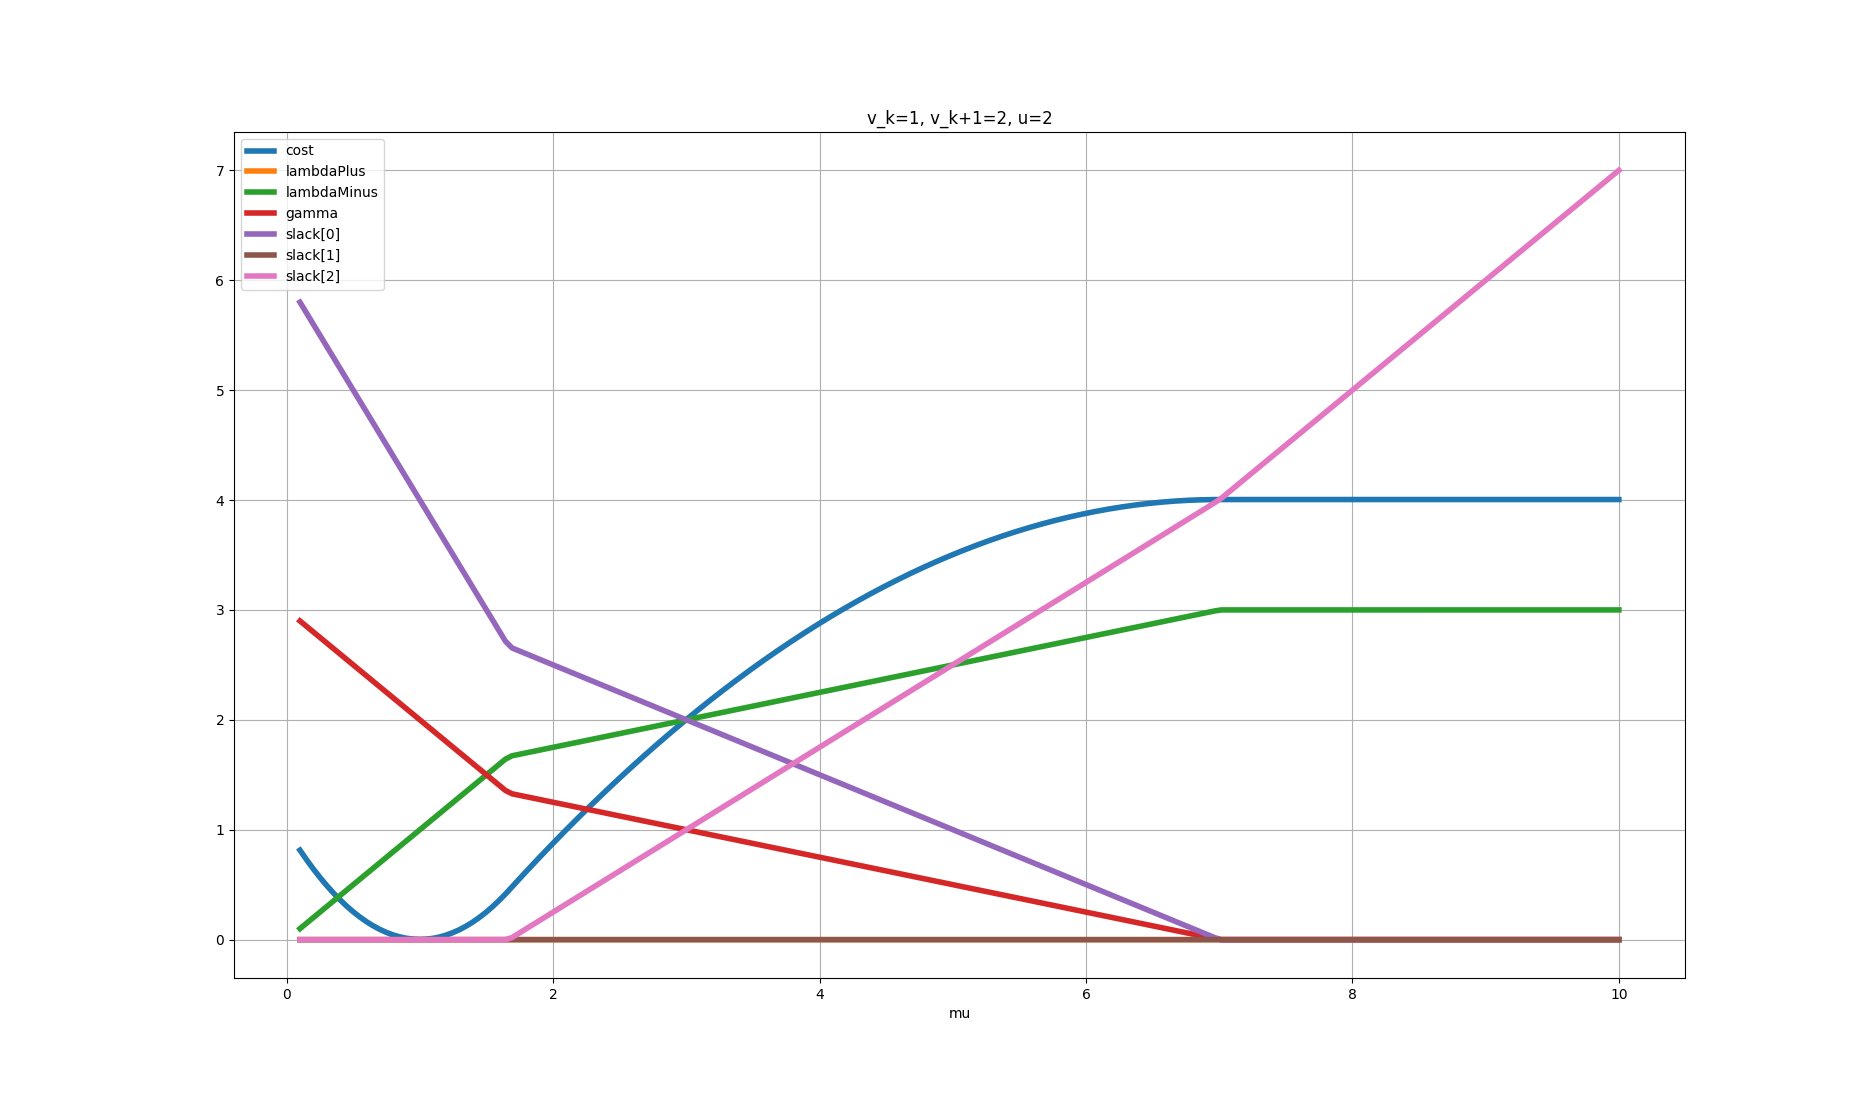
\includegraphics[width=0.9\textwidth]{experiment1}
\end{figure}

\textbf{Soft complimentarity, soft nonnegativity, hard lambda}
\begin{figure}[H]
    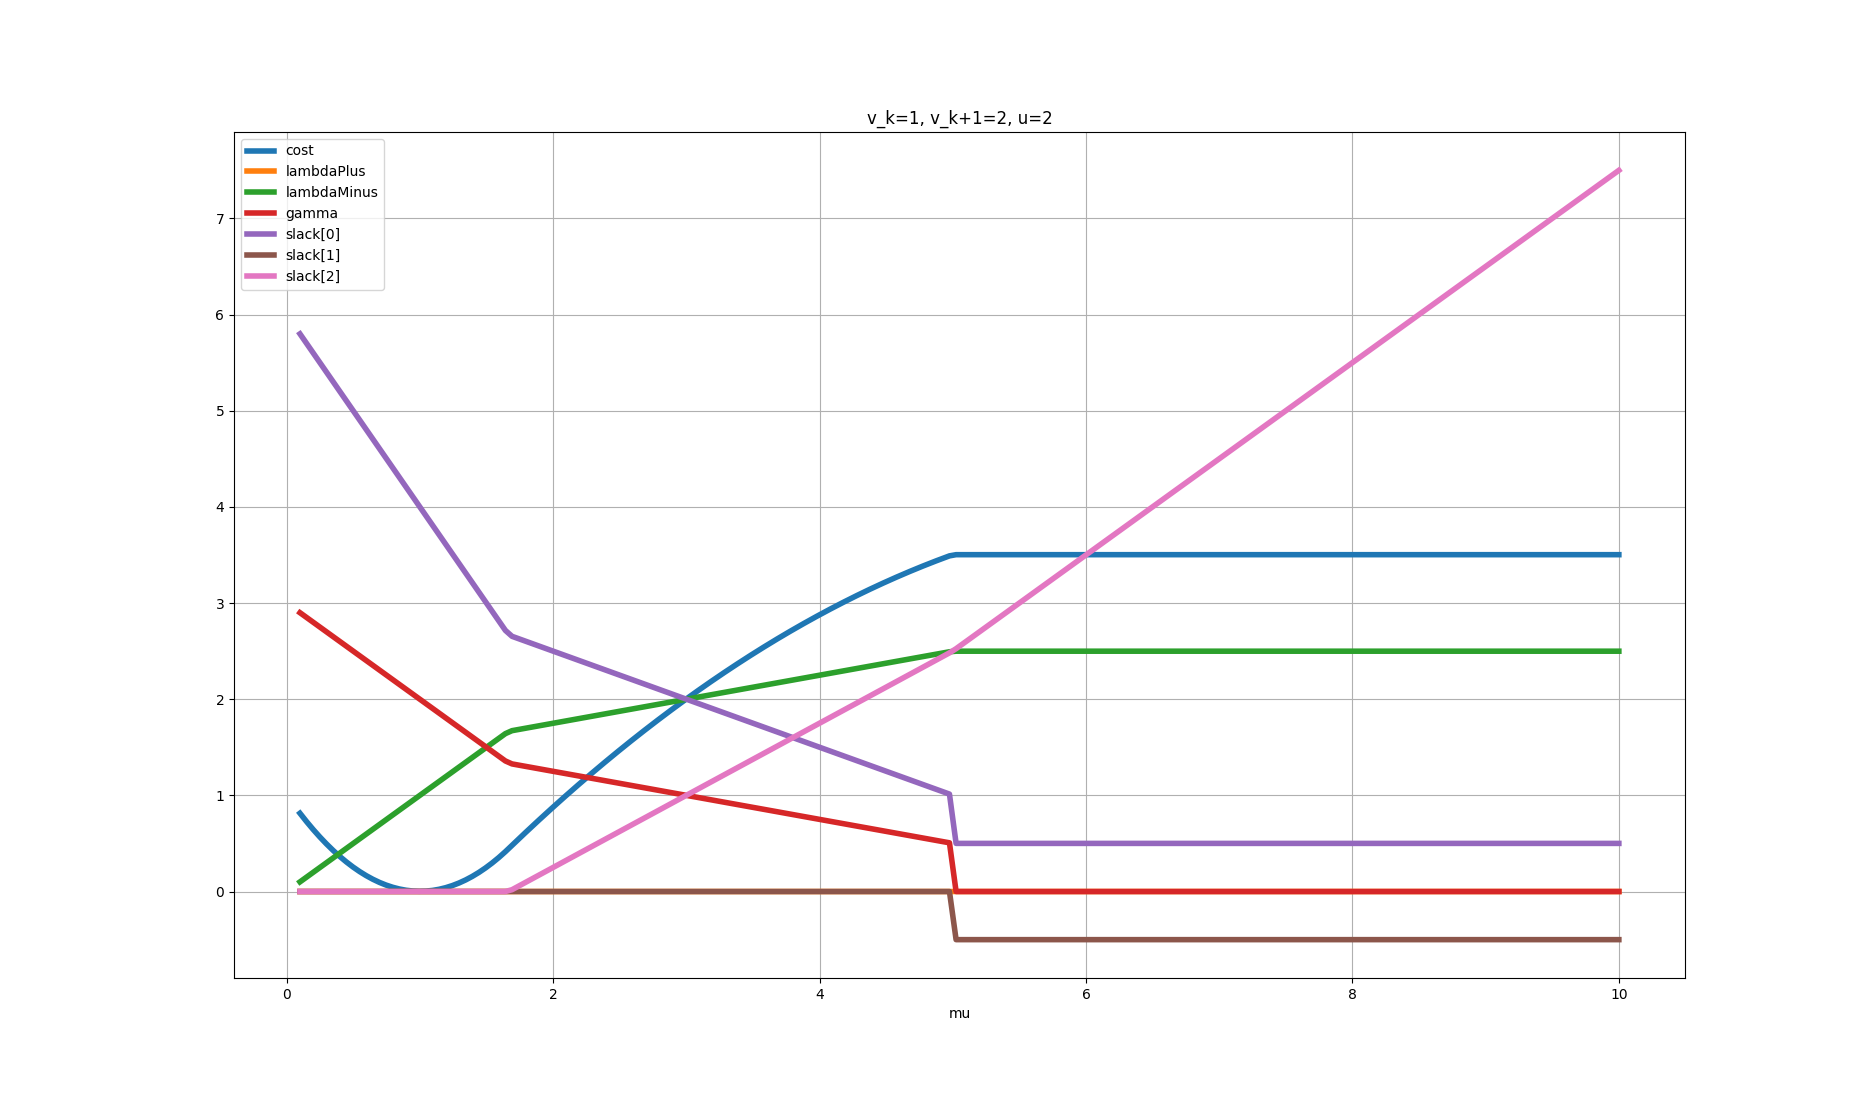
\includegraphics[width=0.9\textwidth]{experiment2}
\end{figure}

\textbf{Soft complimentarity, hard nonnegativity, soft lambda}
\begin{figure}[H]
    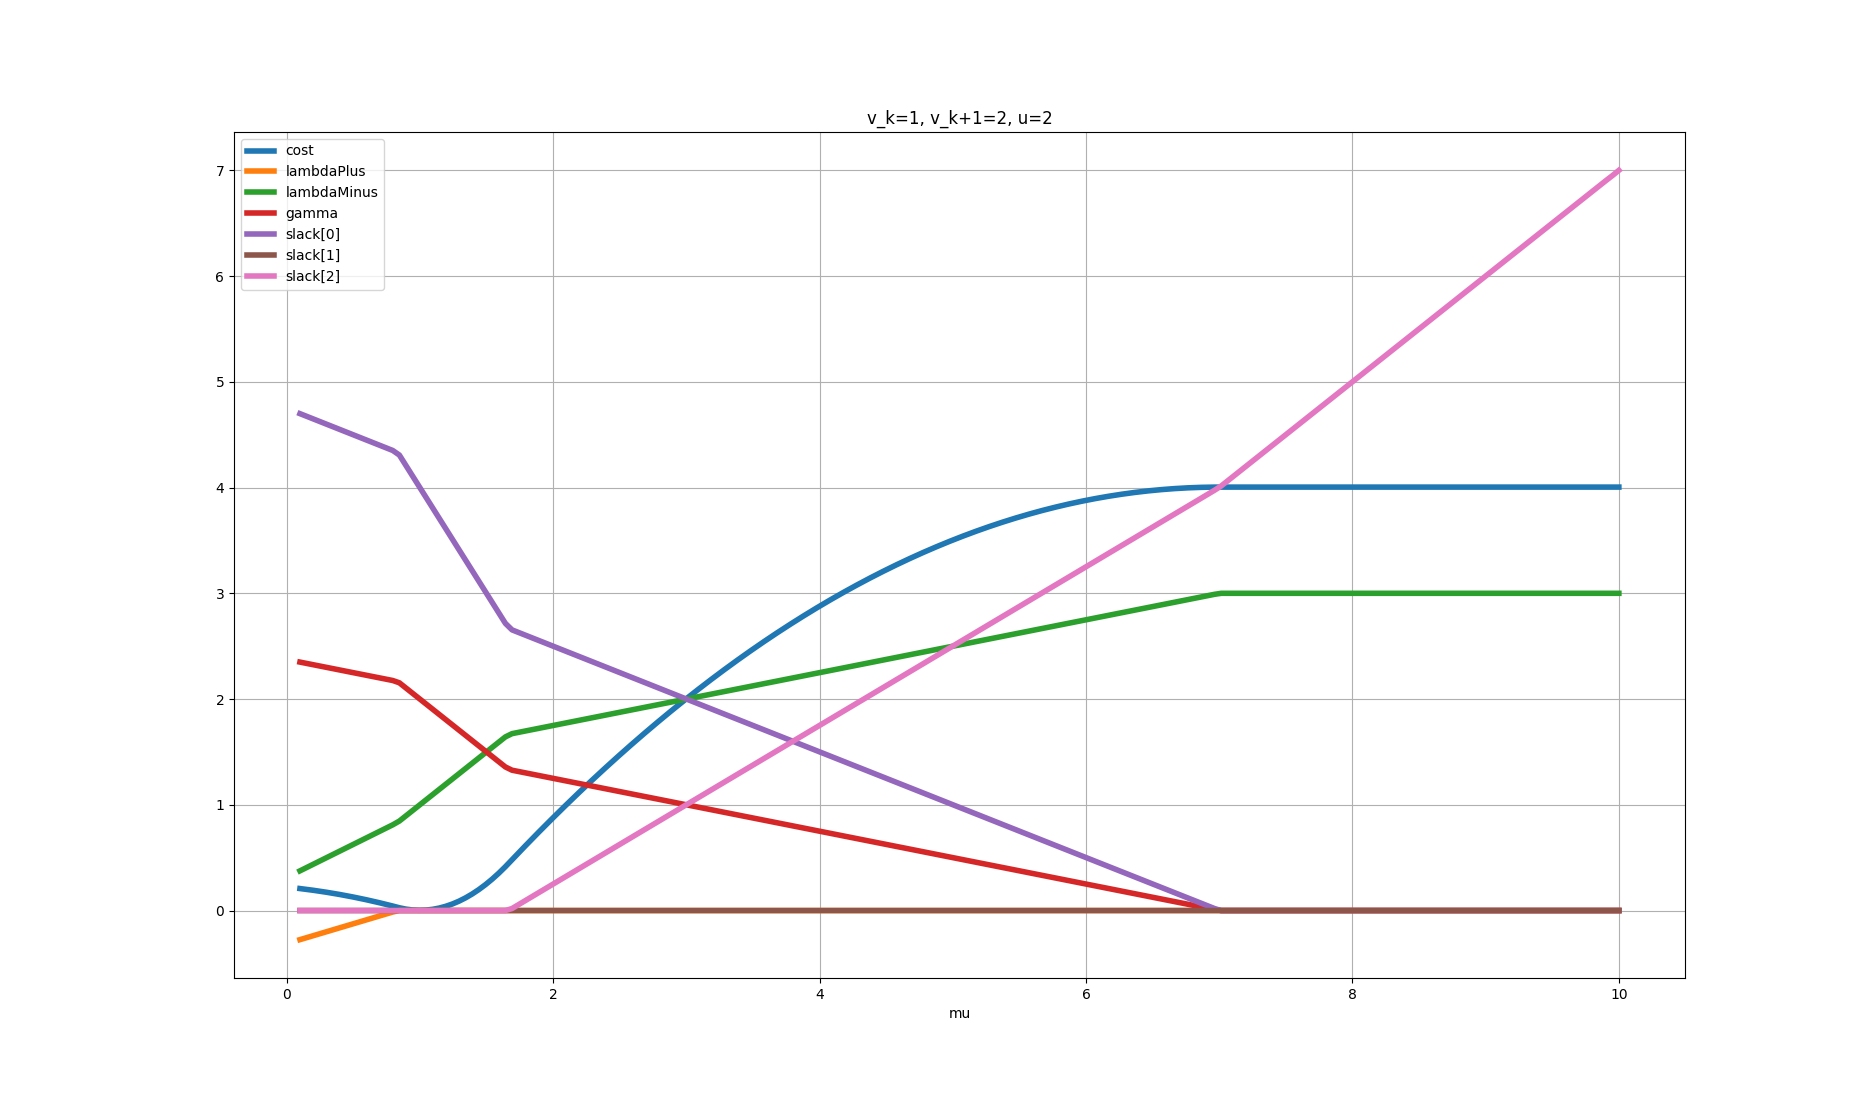
\includegraphics[width=0.9\textwidth]{experiment3}
\end{figure}

\section{Random ideas}
\begin{itemize}
    \item Markov random field / Markov chain for state transitions. Captures multimodality. However, continuous and multidimensional state space is an issue. Could potentially use stick/slip/detach as states instead.
    \item Generalizing direct formulation to non-full-rank jacobian scenarios
    \item Relu into each element of $M$ (one pos, one neg) -> learn exact zeros in $M$
    \item Use gamma to determine sticking? Doesn't actually work that well
    \item Learn $D$ matrix!
    \item For bilevel optimization idea: encode inner soft constraints function as KKT equality conditions, then just impose these as conditions on the higher level optimization problem.
\end{itemize}
\end{document}
